% Insert after VI-D. Requires graphicx. Copy figures/ next to the manuscript.
\subsection{Timing Fidelity and Simulation Cost}
Production execution uses native NetSquid 1.1.7 \texttt{QuantumProgram}s:
CNOT, H, and two sequential measurements for BSM, followed at the destination
by X-or-I and Z-or-I correction slots. Each physical instruction has a configured
duration. Native program-done callbacks release execution resources and trigger
Q2NS completion; BSM completion creates the actual R--B UDP packet at that time.
Native T1/T2 models account for both idle storage and active instruction time;
ideal gates act at instruction completion. These durations are illustrative
model parameters rather than hardware calibration.

Before session execution, pre-generated EPR halves are delivered by native
NetSquid quantum channels from R to A and B, with delays 0.8 and 1.2 ms.
The remote qubits enter destination memory only on port reception. R learns
readiness with ideal zero delay; loss and heralding are outside this model.
All variants retain these channels, memory noise and resource-ready gating.
No-Dq-R changes only R execution capacity; Fixed-Dc changes only result transport.
Latency includes resource wait from the original local session start.

A separately implemented NetSquid-only channel and timed circuit enumerates the four BSM
outcomes with Born probabilities. For each execution model, we compare the
observed branch's intermediate gate states and frame, packet-arrival,
correction-start and usable states using that model's operation timestamps.
This checks the implementation of the configured circuit/noise model; it does
not claim equivalence to physical hardware or the earlier atomic state model.
An independent analytic resource-ready/FIFO schedule also checks start, completion and waiting
times for 500 R/B requests in 12 mixed-protocol runs, with maximum error 0 ns.

For simulation cost, we execute finite mixed Swap--Teleport batches of
1, 4, 8, 16, 32, and 64 sessions with a request interval of 0.8 ms, at
R--B background offered loads of 0 and 0.70. Each condition has one warmup
and ten measured repetitions in shuffled order. All runs retain native memory
noise, instruction-state probes, production event logging, and the full background-traffic drain.
Runtime includes state initialization, ns-3 startup/configuration, federation,
and shutdown, but excludes build/import time, offline independent-reference
validation, and result-file writing. All repeated traces are identical within
each condition and pass packet, resource, clock, and quantum-state validation.
The error bars in Fig.~\ref{fig:timing-cost}(b) are 95\% bootstrap intervals
over runtime repetitions, not over network workloads. These measurements
characterize finite-batch cost on a fixed topology, rather than isolated IPC
overhead or arbitrary-topology scalability.

At 64 sessions, mean total simulation runtimes are 2.18 [1.96, 2.41] and 2.81 [2.36, 3.34] s at offered loads 0 and 0.70, respectively. The corresponding synchronization-round counts are 451 and 850, and bidirectional IPC line counts are 2609 and 4338. Counts include setup and the complete traffic drain.

\begin{figure*}[t]
\centering
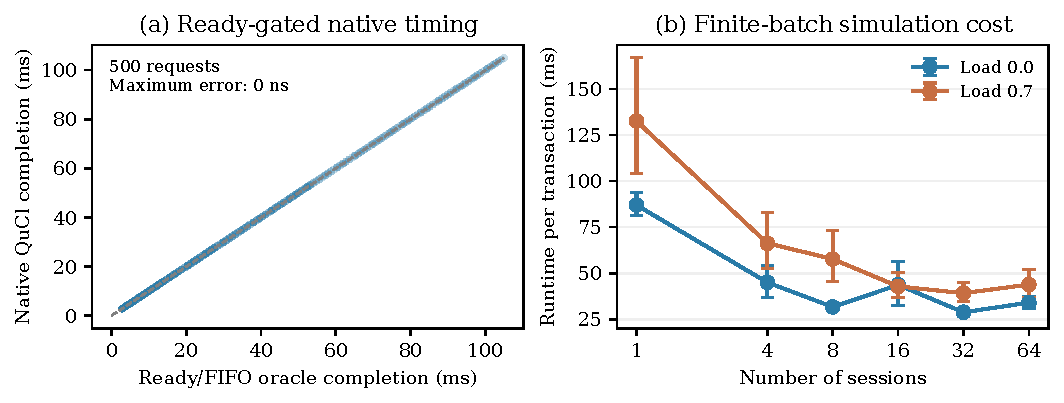
\includegraphics[width=\textwidth]{figures/fig7-timing-cost.pdf}
\caption{Additional validation. (a) Actual native circuit completion timing against an
independent analytic FIFO schedule. (b) Mean simulation
runtime per completed transaction, with 95\% repetition-bootstrap intervals.
Offline reference validation and file writing are excluded.}
\label{fig:timing-cost}
\end{figure*}
